\documentclass[16pt,a4paper]{article}
\usepackage[utf8]{inputenc}
\usepackage{graphicx}
\usepackage[left=2cm,right=2cm,top=2cm,bottom=2cm]{geometry}
\author{Andrea Colarieti Tosti}
\title{Betriebsysteme Blatt 1 Lösung}


\begin{document}
\maketitle
 \section*{Aufgabe 4}

 \paragraph*{a)}
 Offene unterprogramme sind für größeren aufgaben uneffizient. Da sie Speicherplatz verschwenden und oft nachträglich geändert werden müssen.
 \paragraph*{b)}
  Der Programmieraufwand und Speicherverbrauch z.B. einer Addition zweier Zahlen
direkt im Code ist geringer als die Rechnung in ein geschlossenes Unterprogramm
auszulagern, für das zusätzlich noch die Sprungbefehle hinzugefügt werden müssen.

 \paragraph*{c)}
 Call by Value und Call by Reference
 \paragraph*{d)}
 Das Statusregister
PC der CPU enthält die Adresse der Speicherzelle
des nächsten auszuführenden Befehls. Ein Sprungbefehl (JMP addr) überschreibt diesen Wert durch eine neue Adresse.
 \paragraph*{e)}
 CALL unterscheidet sich von JMP durch die zusätliche sicherung der Rücksprungadresse.
 \paragraph*{f)}
 Die Rückkehradresse für das RET befehl kann sich an zwei Stellen befinden:\\ Im register RA oder \\
 auf dem Stack.
 \section*{Aufgabe 5}
 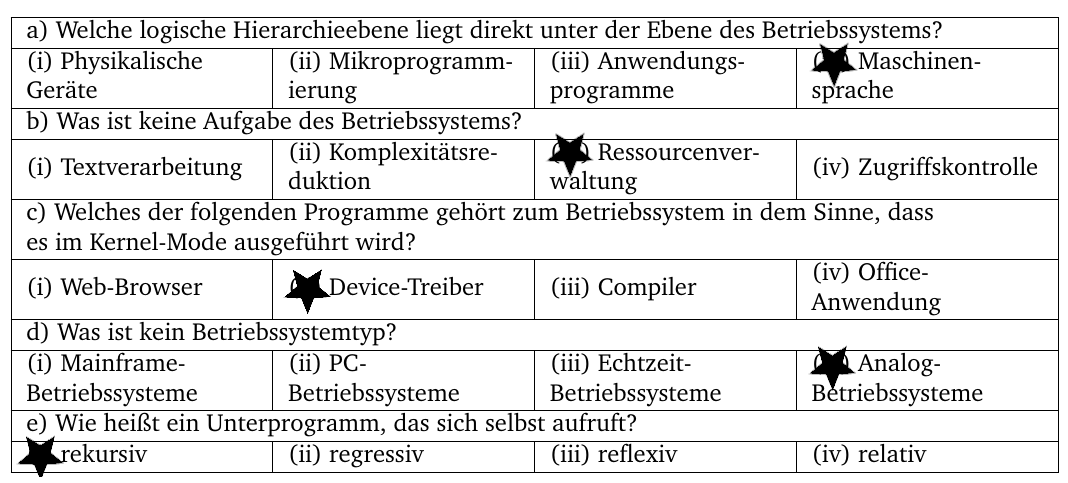
\includegraphics[scale=1.8]{multichoice.png} 
	
\end{document}